\chapter{\label{ch_lcm}The LCM Contention Manager}
\markright{Mohammed El-Shambakey \hfill Chapter~\ref{ch_lcm}. LCM \hfill}
%
Under ECM and RCM (Chapter~\ref{ecm-rcm}), each atomic section can be aborted for at most $2s_{max}$ by a single interfering atomic section. We present a novel contention manager (CM) for resolving transactional conflicts, called length-based CM (or LCM)~\cite{lcmdac2012}. LCM can reduce the abortion time of a single atomic section due to an interfering atomic section below $2s_{max}$. We upper bound transactional retries and response times under LCM, when used with G-EDF and G-RMA schedulers. We identify the conditions under which LCM outperforms ECM, RCM, retry-loop lock-free~\cite{key-5} and real-time locking protocols (i.e., OMLP\cite{springerlink:10.1007/s10617-012-9090-1,key-3} and RNLP\cite{6257574}).

The rest of this Chapter is organized as follows: Section~\ref{sec:lcm} presents Length-based Contention Manager (LCM) and illustrates its behaviour. Section~\ref{sec:lcm_properties} derives LCM properties. Retry cost and response time analysis of tasks under G-EDF/LCM is given in Section~\ref{response g-edf/lcm}. Schedulability of G-EDF/LCM is compared to schedulability of ECM, lock-free and locking protocols in Section~\ref{performance g-edf-lcm}. Section~\ref{rma} gives retry cost and response time analysis for G-RMA/LCM. Schedulability of G-RMA/LCM is compared against RCM, lock-free and locking protocols in Section~\ref{rma eval}. We conclude Chapter in Section~\ref{sec:conclusions_lcm}.
%
\section{\label{sec:lcm}Length-based CM}
%
LCM resolves conflicts based on the priority of conflicting transactions, besides the length of the interfering atomic section, and the length of the interfered atomic section. Priority of each transaction equals priority of its containing job (i.e., $p\left(s_i^k\right)=p_i^x$ where $s_i^k \in \tau_i^x$). ECM and RCM (Chapter~\ref{ecm-rcm}) use only priorities to resolve conflicts. LCM allows lower priority jobs to retry for lesser time than that under ECM and RCM, but higher priority jobs, sometimes, wait for lower priority ones with bounded priority-inversion.

\subsection{\label{sec 9.1}Design and Rationale}
%
\begin{algorithm}
\footnotesize{
\LinesNumbered
\KwData{$s_i^k$ and $s_j^l$ are two conflicting atomic sections.\\$\psi\rightarrow$ predefined threshold $\in [0,1]$.\\$\delta_i^k \rightarrow$ remaining execution length of $s_i^k$.\\
$s\left(s_i^k\right) \rightarrow$ start time of $s_i^k$. $s\left(s_i^k\right)$ is updated each time $s_i^k$ aborts and retries to the start time of the new retry.\\
$s\left(s_j^l\right) \rightarrow$ the same as $s\left(s_i^k\right)$ but for $s_j^l$.
}
\KwResult{which atomic section of $s_i^k$ or $s_j^l$ aborts}
\eIf{$s\left(s_i^k\right) < s\left(s_j^l\right)$\label{lcm:s_i_k start before s_j_l}}
{
\eIf{$p\left(s_i^k\right) > p\left(s_j^l\right)$}
	{$s_j^l$ aborts\label{lcm:step_sicommits}\;}
	{$c_{ij}^{kl}=len(s_j^l)/len(s_i^k)$\label{step_cijkl}\;
	$\alpha_{ij}^{kl}=ln(\psi)/(ln(\psi)-c_{ij}^{kl})$\label{step_alphaijkl}\;
	$\alpha=\left(len(s_i^k)-\delta_i^k\right)/len(s_i^k)$\label{step_alpha}\;
	\eIf{$\alpha \le \alpha_{ij}^{kl}$}
	{$s_i^k$ aborts\label{lcm:step_siaborts}\;}
	{$s_j^l$ aborts\label{step_sjaborts}\;}
	}
	}
	{
	Swap $s_i^k$ and $s_j^l$\label{lcm:s_j_l start before s_i_k}\;
	}
	}
\caption{LCM}
\label{alg_lcm}
\end{algorithm}
%
For both ECM and RCM, $s_{i}^{k}$ can be totally repeated if $s_{j}^{l}$ --- which belongs to a higher priority job $\tau_{j}^b$ than $\tau_{i}^a$ --- conflicts with $s_{i}^{k}$
at the end of its execution, while $s_{i}^{k}$ is just about
to commit. Thus, LCM, shown in Algorithm~\ref{alg_lcm}, uses the remaining length of $s_{i}^{k}$ when it is interfered,
as well as $len(s_{j}^{l})$, to decide which transaction must be aborted. If $s_i^k$ starts before $s_j^l$, then $s_i^k$ is the interfered atomic section and $s_j^l$ is the interfering atomic section (step~\ref{lcm:s_i_k start before s_j_l}). Otherwise, $s_i^k$ and $s_j^l$ are swapped (step~\ref{lcm:s_j_l start before s_i_k}). If $p\left(s_i^k\right)$ was greater than $p\left(s_j^l\right)$, then $s_i^k$ would be the one that commits, because it belongs to a higher priority job, and it started before $s_j^l$ (step~\ref{lcm:step_sicommits}). Otherwise, $c_{ij}^{kl}$ is calculated (step~\ref{step_cijkl}) to determine whether it is worth aborting $s_i^k$ in favour of $s_j^l$, because $len(s_j^l)$ is relatively small compared to the remaining execution length of $s_i^k$ (explained further).

We assume that:
\begin{equation}
c_{ij}^{kl}=len(s_{j}^{l})/len(s_{i}^{k})
\label{cm_eq}\end{equation}
where $c_{ij}^{kl}\in]0,\infty[$, to cover all possible lengths of $s_{j}^{l}$.
Our idea is to reduce the opportunity for the abort of $s_{i}^{k}$ if it is close to committing when interfered and $len(s_{j}^{l})$ is large. This abort opportunity is increasingly reduced as $s_{i}^{k}$ gets closer to the end of its execution, or $len(s_{j}^{l})$ gets larger. 

On the other hand, as $s_{i}^{k}$ is interfered early,
or $len(s_{j}^{l})$ is small compared to $s_{i}^{k}$'s remaining length, the abort opportunity 
is increased even if $s_i^k$ is close to the end of its execution. To decide whether $s_{i}^{k}$ must be aborted or not, we use a threshold value $\psi\in[0,1]$ that determines $\alpha_{ij}^{kl}$ (step~\ref{step_alphaijkl}), where $\alpha_{ij}^{kl}$ is the maximum percentage of $len(s_i^k)$ below which $s_j^l$ is allowed to abort $s_i^k$ and is calculated as 
%
\begin{equation}
\alpha_{ij}^{kl}=\frac{ln\left(\Psi\right)}{ln\left(\Psi\right)-c_{ij}^{kl}}
\label{eq:lcm_alpha_ij_kl}
\end{equation}
%
Thus, if the already executed part of $s_i^k$ --- when $s_j^l$ interferes with $s_i^k$ --- does not exceed $\alpha_{ij}^{kl}len(s_i^k)$, then $s_i^k$ is aborted (step~\ref{lcm:step_siaborts}). Otherwise, $s_j^l$ is aborted (step~\ref{step_sjaborts}).
%
\begin{figure}[htbp]
\centering
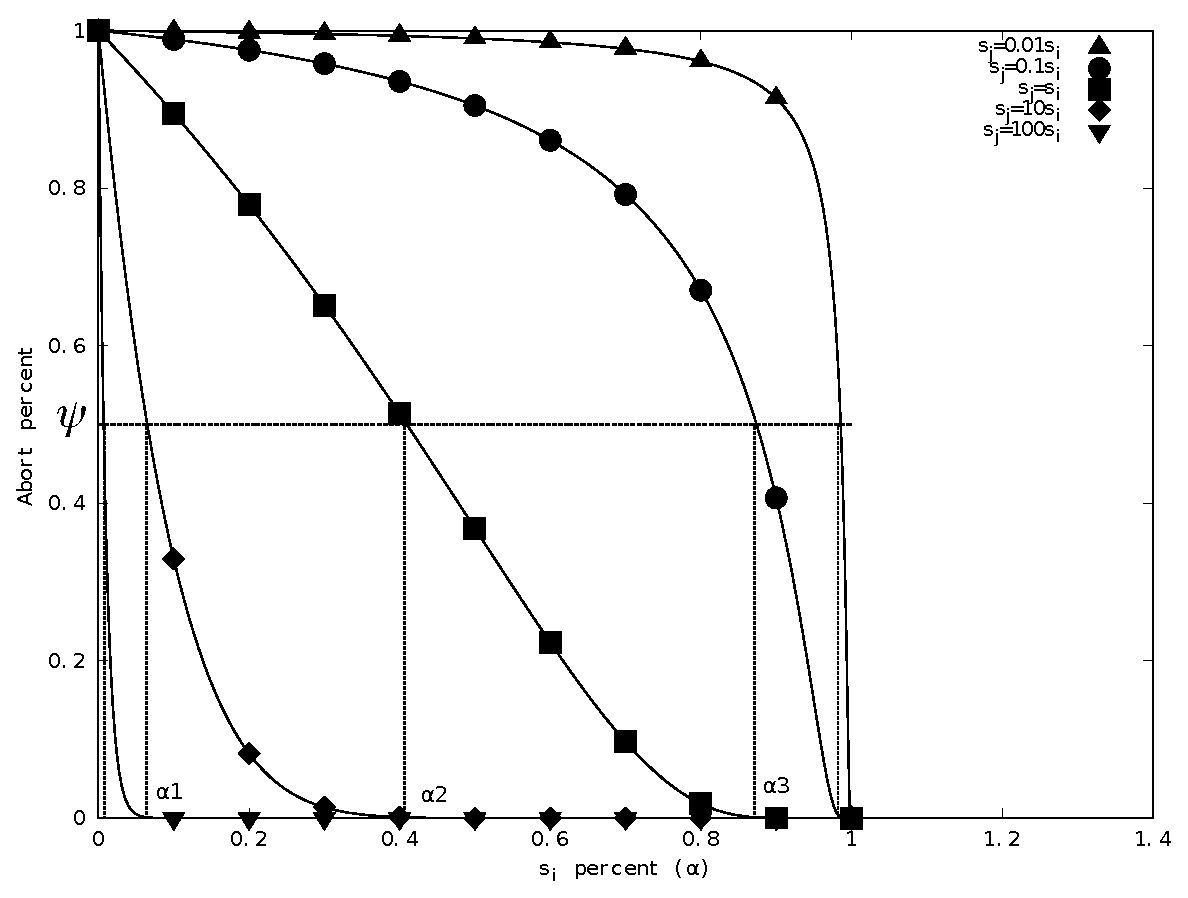
\includegraphics[scale=0.4]{figures/figure16}
\caption{\label{fig16}Interference of $s_{i}^{k}$ by various lengths of 
$s_{j}^{l}$}
\end{figure}

The behaviour of LCM is illustrated in Figure~\ref{fig16}. In this figure, the horizontal axis corresponds to different values of $\alpha$ ranging from $0$ to $1$, and the vertical axis corresponds to different values of abort opportunities, $f(c_{ij}^{kl},\alpha)$, ranging from $0$ to $1$ and calculated by~(\ref{eq49}):
\begin{equation}
f(c_{ij}^{kl},\alpha)=e^{\frac{-c_{ij}^{kl}\alpha}{1-\alpha}}
\label{eq49}\end{equation}
where $c_{ij}^{kl}$ is calculated by~(\ref{cm_eq}).

Figure~\ref{fig16} shows one atomic section $s_i^k$ (whose $\alpha$ changes along the horizontal axis) interfered by five different lengths of $s_j^l$.
For a predefined value of $f(c_{ij}^{kl},\alpha)$ (denoted as $\psi$ in Algorithm~\ref{alg_lcm}), there corresponds a specific value of $\alpha$ (which is $\alpha_{ij}^{kl}$ in Algorithm~\ref{alg_lcm}) for each curve. For example, when $len(s_j^l)=0.1 \times len(s_i^k)$, $s_j^l$ aborts $s_i^k$ if the latter has not executed more than $\alpha3$ percentage (shown in Figure~\ref{fig16}) of its execution length. As $len(s_{j}^{l})$ decreases, the corresponding $\alpha_{ij}^{kl}$ increases (as shown in Figure~\ref{fig16}, $\alpha3>\alpha2>\alpha1$).

Equation (\ref{eq49}) achieves the desired requirement that the abort opportunity is reduced as $s_{i}^{k}$ gets closer to the end of its execution (as $\alpha\rightarrow1,\, f(c_{ij}^{kl},1)\rightarrow0$),
or as the length of the conflicting transaction increases (as $c_{ij}^{kl}\rightarrow\infty,\, f(\infty,\alpha)\rightarrow0$). Meanwhile, this abort opportunity is increased as $s_{i}^{k}$ is interfered closer to its release (as $\alpha\rightarrow0,\, f(c_{ij}^{kl},0)\rightarrow1$),
or as the length of the conflicting transaction decreases (as $c_{ij}^{kl}\rightarrow0,\, f(0,\alpha)\rightarrow1$).

LCM is not a centralized CM, which means that, upon a conflict, each transactions has to decide whether it must commit or abort. LCM suffers from transitive retry (Section~\ref{subsec:ecm_transitive_retry}).
%
\begin{clm}\label{clm:lcm-transitive-retry}
LCM suffers from transitive retry for multi-object transactions.
\end{clm}
%
\begin{proof}\normalfont
%
Following the proof of Claim~\ref{ecm-rcm-transitive-retry}, Claim follows.
%
\end{proof}
%
\subsection{LCM Illustrative Example}
%
Behaviour of LCM can be illustrated by the following example:
\begin{itemize}
\item Transaction $s_{i}^{k}\in\tau_{i}^{x}$ begins execution.
Currently, $s_{i}^{k}$ does not conflict with any other transaction.
\item Transaction $s_{j}^{l}\in\tau_{j}^{y}$ is released while
$s_{i}^{k}$ is still running. $\Theta_i^{k^{ex}} \cap \Theta_j^l \neq \emptyset$ and $p_{j}^{y}>p_{i}^{x}$ (where priority is dynamic in G-EDF, and fixed in G-RMA). $c_{ij}^{kl}$,
$\alpha_{ij}^{kl}$ and $\alpha$ are calculated by steps~\ref{step_cijkl} to~\ref{step_alpha} 
in Algorithm~\ref{alg_lcm}. $s_{i}^{k}$ has not reached $\alpha$
percentage of its execution length yet. 
\item $\alpha<\alpha_{ij}^{kl}$. Then, $s_{j}^{l}$ is allowed
to abort and restart $s_{i}^{k}$.
\item $s_{j}^{l}$ commits. $s_{i}^{k}$ executes again.
\item Transaction $s_{h}^{v}\in\tau_{h}^{u}$ is released while
$s_{i}^{k}$ is running. $\Theta_i^{k^{ex}} \cap \Theta_h^v \neq \emptyset$ and $p_{h}^{u}>p_{i}^{x}$. $c_{ih}^{kv}$,
$\alpha_{ih}^{kv}$ and $\alpha$ are calculated by steps~\ref{step_cijkl} to~\ref{step_alpha}
in Algorithm~\ref{alg_lcm}. $s_{i}^{k}$ has already passed $\alpha$
percentage of its execution length. So, $s_{h}^{v}$ aborts
and restarts in favour of $s_{i}^{k}$.
\item Transaction $s_{a}^{b}\in\tau_{a}^{f}$ is released. $\Theta_i^{k^{ex}} \cap \Theta_a^b \neq \emptyset$ and $p_{a}^{f}>p_{i}^{x}$
but $p_{a}^{f}<p_{h}^{u}$. $c_{ia}^{kb}$, $\alpha_{ia}^{kb}$
and $\alpha$ are calculated by steps~\ref{step_cijkl} to~\ref{step_alpha} in Algorithm~\ref{alg_lcm}.
$s_{i}^{k}$ has not reached $\alpha$ percentage of its execution
length yet. So, $s_{a}^{b}$ is allowed to abort $s_{i}^{k}$.
Because $s_{a}^{b}$ is just starting, LCM allows $s_{h}^{v}$
to abort $s_{a}^{b}$. So, the highest priority transaction
is not blocked by an intermediate priority transaction $s_{a}^{b}$.
\item When $s_{h}^{v}$ commits. $s_{a}^{b}$ is allowed
to execute while $s_{i}^{k}$ is retrying.
\item When $s_{a}^{b}$ commits, $s_{i}^{k}$ executes.
\item Transaction $s_{c}^{n}\in\tau_{o}^{z}$ is released while
$s_{i}^{k}$ is running. $\Theta_i^{k^{ex}} \cap \Theta_c^n \neq \emptyset$ and $p_{o}^{z}<p_{i}^{x}$. So, $s_{i}^{k}$
commits first, then $s_{c}^{n}$ is allowed to proceed.
\end{itemize} 
%
\section{Properties}\label{sec:lcm_properties}
%
LCM properties are given by the following Lemmas. These properties are used to derive retry cost and response time of transactions and tasks under LCM.
%
\begin{clm}\label{clm:lcm_deadlock_avoid}
%
$r\left(s_i^k\right)$ is updated each time $s_i^k$ aborts and retries to the new start time of the new retry to avoid deadlock that can result from conflicting transactions aborting each other.
%
\end{clm}
%
\begin{proof}
%
Assume a set of transactions $S$ that are conflicting together. Each transaction aborts and retries due to the others. So, a higher priority transaction $s_j^l$ aborts and retries due to a lower priority transaction $s_i^k$. $s_i^k$ itself aborts and retries due to another transaction. Thus, the new $r\left(s_i^k\right)$ will be at least equal to the new $r\left(s_j^l\right)$. By definition of LCM, $s_j^l$ will be chosen to commit first because of its higher priority. By extending this result to all transactions in $S$, the highest priority transaction will commit. Thus, deadlock is avoided. Claim follows.
%
\end{proof}
%
\begin{clm}\label{LCM_higher_rc}
%
Let $s_{j}^{l}$ interferes once with $s_{i}^{k}$ at most at $\alpha_{ij}^{kl}$. $p\left(s_j^l\right) > p\left(s_i^k\right)$. Then, the maximum contribution of $s_{j}^{l}$ to 
$s_{i}^{k}$'s retry cost is:
\begin{equation}
W_i^k(s_j^l)\le \alpha_{ij}^{kl}len\Big(s_{i}^{k}\Big)+len\Big(s_{j}^{l}\Big)\label{eq47}\end{equation}
%
\end{clm}
%
\begin{proof}\normalfont
%
If $s_{j}^{l}$ interferes with $s_{i}^{k}$ at a $\Upsilon$ percentage, where $\Upsilon<\alpha_{ij}^{kl}$,
then the retry cost of $s_{i}^{k}$ is $\Upsilon len(s_{i}^{k})+len(s_{j}^{l})$, which is lower than that calculated in (\ref{eq47}). Besides, 
if $s_{j}^{l}$ interferes with $s_{i}^{k}$ after
$\alpha_{ij}^{kl}$ percentage, then $s_{i}^{k}$ will not
abort.
%
\end{proof}
%
\begin{clm}\label{LCM_lower_rc}
%
A higher priority transaction, $s_j^l$, aborts and retries due to a lower priority transaction, $s_i^k$, if $s_{j}^{l}$ interferes with $s_{i}^{k}$ after the $\alpha_{ij}^{kl}$ percentage. $s_j^l$'s retry cost, due to $s_{i}^{k}$ is upper bounded by:
%
\begin{equation}
W_j^l(s_i^k)\le \Big(1-\alpha_{ij}^{kl}\Big)len\Big(s_{i}^{k}\Big)
\label{eq48}
\end{equation}
%
\end{clm}
%
\begin{proof}\normalfont
It is derived directly from Claim~\ref{LCM_higher_rc}, as $s_j^l$ will have to retry for the remaining length of $s_i^k$.
\end{proof}
%
\begin{clm}\label{clm:alpha_increase_with_max_interfered}
As length of $s_i^k$- interfered by a higher priority transaction $s_j^l$ - increases, then $\alpha_{ij}^{kl}$ also increases.
\end{clm}
%
\begin{proof}\normalfont
%
As $len\left(s_i^k\right)$ increases, then $c_{ij}^{kl}$ decreases by definition of (\ref{cm_eq}). Noting that $ln(\Psi) \le 0$ because $\Psi \in [0,1]$. Thus, $\alpha_{ij}^{kl}$ increases as $c_{ij}^{kl}$ decreases by definition of (\ref{eq:lcm_alpha_ij_kl}). Claim follows.
%
\end{proof}
%
\begin{clm}\label{clm:lcm_effect_one_tx_in_rc_multiple_txs_higher_priority}
%
Let $conf\left\{ s_{i}^{k}\right\} $ be the set of all transactions
that do not belong to any job of $\tau_{i}$ and are conflicting, directly or indirectly(transitively), with
$s_{i}^{k}$. Each transaction $s_{j}^{l}\in conf\left\{ s_{i}^{k}\right\},\,p\left(s_j^l\right)>p\left(s_i^k\right) $
contributes to the retry cost of $s_{i}^{k}$ by at most 
\begin{equation}
len\left(s_{j}^{l}+\alpha_{max}^{jl}s_{max}(\Theta)\right)\label{eq:lcm_effect_one_tx_in_rc_multiple_txs_higher_priority}
\end{equation}
where $s_{max}(\Theta)$ is the maximum length atomic section
(transaction) in $conf\{s_{i}^{k}\}$ that accesses at least one object in $\Theta$ and its priority is lower than $p(s_{j}^{l})$. $s_{max}\left(\Theta\right) \not\in s_{j}$ and $\Theta\subseteq\Theta_{i}^{k^{ex}}\cap\Theta_{j}^{l}$. $\alpha_{max}^{jl}$ is calculated by (\ref{eq:lcm_alpha_ij_kl}) due to interference of $s_{max}\left(\Theta\right)$ by $s_j^l$.
%
\end{clm}
%
\begin{proof}
Under ECM and RCM (Chapter~\ref{ecm-rcm}), lower priority transactions abort and retry only due to higher priority transactions. Whereas, under LCM, a transaction $s_i^k$ can be aborted due to higher priority transactions. $s_i^k$ can also be delayed by lower priority transactions. Thus, proof follows proof of Claim~\ref{clm:effect_one_tx_in_rc_multiple_txs} with the following modifications:
\begin{compactitem}
\item According to Claims~\ref{LCM_higher_rc} and~\ref{LCM_lower_rc}, $s_j^l$ can cause lower priority transactions to retry and higher priority transactions to be delayed. From Claims~\ref{LCM_higher_rc} and~\ref{LCM_lower_rc}, it appears that contribution of $s_j^l$ to the retry cost of lower priority transactions is greater than delay caused by $s_j^l$ to higher priority transactions. Thus, retry cost caused by $s_j^l$ to lower priority transactions is taken as the contribution of $s_j^l$ to the retry cost of $s_i^k$.
\item By Claim~\ref{clm:alpha_increase_with_max_interfered} and definition of $s_{max}\left(\Theta\right)$, $\alpha_{max}^{jl}$ is the maximum $\alpha$ that results from interference of a lower priority transaction- accessing any object $\theta \in \Theta$ - by $s_j^l$.
\item $s_i^k$ can abort and retry due to higher priority transactions. Also, $s_i^k$ can be delayed due to lower priority transactions. Thus, $p\left(s_{max}\right)<p\left(s_j^l\right)$, but $p\left(s_{max}^{jl}\right)$ does not have to be greater than $p\left(s_i^k\right)$.
\end{compactitem}
Claim follows.
%
\end{proof}
%
\begin{clm}\label{clm:lcm_effect_one_tx_in_rc_multiple_txs_lower_priority}
%
Let $conf\left\{ s_{i}^{k}\right\} $ be the set of all transactions
that do not belong to any job of $\tau_{i}$ and are conflicting, directly or indirectly(transitively), with
$s_{i}^{k}$. Each transaction $s_{j}^{l}\in conf\left\{ s_{i}^{k}\right\},\,p\left(s_j^l\right)<p\left(s_i^k\right) $
contributes to the delay of $s_{i}^{k}$ by at most 
\begin{equation}
\left(1-\alpha_{min}^{jl}\right)len\left(s_j^l\right)
\label{eq:lcm_effect_one_tx_in_rc_multiple_txs_lower_priority}
\end{equation}
where $\alpha_{min}^{jl}$ is the minimum $\alpha_{jx}^{ly}$- calculated by (\ref{eq:lcm_alpha_ij_kl})- that results from delay of any higher priority transaction $s_x^y$ by the lower priority $s_j^l$.
%
\end{clm}
%
\begin{proof}
%
If $s_j^l$ is to abort and retry, then the delay to $s_i^k$ that results from each retry of $s_j^l$ is covered by Claim~\ref{clm:lcm_effect_one_tx_in_rc_multiple_txs_higher_priority}. Thus, the delay that results from $s_j^l$ when it does not retry is given by Claim~\ref{LCM_lower_rc} by minimizing $\alpha_{ij}^{kl}$ in (\ref{eq48}) to its minimum value (i.e., $\alpha_{min}^{jl}$). Claim follows.
%
\end{proof}
%
\begin{clm}
\label{no priority inversion in lcm}
%
Under LCM with G-EDF and G-RMA, priority inversion time for any job $\tau_i^x$ during $T_i$ is bounded.
\end{clm}
%
\begin{proof}\normalfont
Under LCM, priority of each transaction $s_i^k$ equals priority of its containing job $\tau_i^x$. Under G-EDF, number of lower priority jobs of $\tau_j$ that are released during $T_i$ is upper bounded by $1$. Under G-RMA, number of lower priority jobs of $\tau_j$ that are released during $T_i$ is upper bounded by $\left\lceil\frac{T_i}{T_j}\right\rceil+1$. Number of transactions is fixed for each job. So, by Claim~\ref{clm:lcm_effect_one_tx_in_rc_multiple_txs_lower_priority}, Claim follows.
%
\end{proof}
%
\section{Retry Cost and Response Time of G-EDF/LCM}\label{response g-edf/lcm}
%
\begin{clm}\label{GEDF/LCM response time}
%
Under G-EDF/LCM, the total retry cost suffered by all transactions in any job $\tau_i^x \in \tau_i$ during interval $L \le T_{i}$ due to direct and indirect conflict with other transactions is upper bounded by:
%
\begin{equation}
RC_i\left(L\right) \le \sum_{\tau_{j}\in\gamma_i^{ex}}\left(g_{ij}^{gedf} \sum_{\forall s_j^l,\,\left(\Theta=\Theta_j^l \cap \Theta_i^{ex}\right) \neq \emptyset} len\left(s_{j}^{l} +
\alpha_{max}^{jl}s_{max}(\Theta)\right)\right)
\label{eq78}
\end{equation}
%
where $s_{max}\left(\Theta\right) \not\in s_j$ and $\alpha_{max}^{jl}$ is given by (\ref{eq:lcm_alpha_ij_kl}) due to interference of the lower priority $s_{max}\left(\Theta\right)$ by the higher priority $s_j^l$. $g_{ij}^{gedf}$ is calculated by (\ref{eq:gedf_max_job_no_interfer_j_i}).
%
\end{clm}
%
\begin{proof}\normalfont
%
From Claims~\ref{LCM_higher_rc} and~\ref{LCM_lower_rc}, it appears that contribution of $s_j^l$ to the retry cost of lower priority transactions is greater than delay caused by $s_j^l$ to higher priority transactions. Thus, retry cost caused by $s_j^l$ to lower priority transactions is taken as the contribution of $s_j^l$ to the retry cost of $s_i^k$. Under G-EDF, priorities are determined by the absolute deadline of the job. Thus, the same transaction $s_j^l$ can be of higher or lower priority than $p\left(s_i^k\right)$ according to the absolute deadline of containing job of $s_j^l$. So, only jobs of $\tau_j \in \gamma_i$ that have an absolute deadline that at most coincides with $d_i^x$ are considered. Thus, delay of lower priority transactions is ignored. Following Claim~\ref{clm:lcm_effect_one_tx_in_rc_multiple_txs_higher_priority} and Claim~\ref{gedf-edf}, Claim follows
%
\end{proof}
%
\begin{clm}\label{clm:gedf_lcm_release_conflict}
%
Under G-EDF/LCM, the total retry cost suffered by all transactions in any job $\tau_i^x \in \tau_i$ during an interval $L \le T_i$ due to release of jobs with higher priority than $\tau_i^x$ is upper bounded by 
\begin{equation}
RC_{i_{re}}(L) \le \sum_{\forall \tau_{j}\in\zeta_{i}}\begin{cases}
\left\lceil \frac{L}{T_{j}}\right\rceil s_{i_{max}} & ,L\le T_{i}-T_{j}\\\\
\left\lfloor \frac{T_{i}}{T_{j}}\right\rfloor s_{i_{max}} & ,L>T_{i}-T_{j}
\end{cases}\label{eq:gedf_lcm_release_conflict}
\end{equation}
%
where $\zeta_i=\{\tau_j:\left(\tau_j \ne \tau_i\right)\wedge \left(D_j < D_i \right)\}$.
\end{clm}
%
\begin{proof}
%
G-EDF/LCM and ECM has the same pattern for release of jobs. Thus, proof is the same as proof of Claim~\ref{clm:ecm_release_conflict}. Claim follows.
%
\end{proof}
%
\begin{clm}\label{clm:gedf_lcm_total_rc}
Under G-EDF/LCM, the total retry cost suffered by all transactions in any job $\tau_i^x \in \tau_i$ during an interval $L\le T_i$ is upper bounded by:
\begin{equation}
RC_{i_{to}}(L)=RC_i(L)+RC_{i_{re}}(L)
\label{eq:gedf_lcm_total_rc}
\end{equation}
where $RC_i(L)$ is the maximum retry cost resulting from conflict between transactions in $\tau_i^x$ and transactions of other jobs. $RC_i(L)$ is calculated by (\ref{eq78}). $RC_{i_{re}}(L)$ is the maximum retry cost resulting from the release of higher priority jobs, which preempt transactions in $\tau_i^x$. $RC_{i_{re}}(L)$ is calculated by (\ref{eq:gedf_lcm_release_conflict}).
%
\end{clm}
%
\begin{proof}
Proof follows directly from Claims~\ref{GEDF/LCM response time},~\ref{clm:gedf_lcm_release_conflict} and proof of Claim~\ref{clm:ecm_total_rc}.
%
\end{proof}
%
\begin{clm}\label{clm:gedf_lcm_response_time_upper_bound}
%
Under G-EDF/LCM, maximum response time of any job $\tau_i^x \in \tau_i$ is upper bounded by Claim~\ref{clm:ecm_response_time_upper_bound} where $RC_{i_{to}}(R_i^{up})$ is upper bounded by (\ref{eq:gedf_lcm_total_rc}).
%
\end{clm}
%
\begin{proof}
%
Proof follows directly from Claim~\ref{clm:gedf_lcm_total_rc} and proof of Claim~\ref{clm:ecm_response_time_upper_bound}.
%
\end{proof}
%
\section{Schedulability of G-EDF/LCM}\label{performance g-edf-lcm}
%
We now compare the schedulability of G-EDF/LCM against ECM (Chapter~\ref{ecm-rcm}), lock-free~\cite{key-5} and locking protocols (i.e., OMLP\cite{springerlink:10.1007/s10617-012-9090-1,key-3} and RNLP\cite{6257574}) to understand when G-EDF/LCM will perform better. 
%
\subsection{G-EDF/LCM versus ECM}\label{subsec:gedf_lcm_vs_ecm}
%
We compare the total utilization of ECM with that of G-EDF/LCM. For each method, we inflate the $c_i$ of each task $\tau_i$ by adding the total retry cost suffered by $\tau_i$. Thus, if method $A$ adds total retry cost $RC_A^{to}(T_i)$ to $c_i$, and method $B$ adds total retry cost $RC_B^{to}(T_i)$ to $c_i$, then the schedulability of $A$ and $B$ are compared as:
%
\begin{eqnarray}
\sum_{\forall \tau_{i}}\frac{c_{i}+RC_A^{to}(T_{i})}{T_{i}} & \le & \sum_{\forall \tau_{i}}\frac{c_{i}+RC_B^{to}(T_{i})}{T_{i}}
\label{eqa}
\end{eqnarray}
%
Equation(\ref{eqa}) holds if 
\begin{equation}
\forall \tau_i,\, RC_A^{to}(T_{i}) \le RC_B^{to}(T_{i})
\label{eq:two_cms_comparison}
\end{equation}
Thus, schedulability is compared by comparing total retry cost added by the synchronization methods to any job of $\tau_i$.
%
\begin{clm}\label{lcm versus ecm}
Schedulability of G-EDF/LCM is always equal or better than ECM.
%
\end{clm}
%
\begin{proof}\normalfont
%
Under ECM, $RC_{ECM}^{to}(T_{i})$ is upper bounded by (\ref{eq:ecm_total_rc_stm_comp}) with replacing $\gamma_i$ by $\gamma_i^{ex}$. 

$RC_{G-EDF/LCM}^{to}(T_i)$ is given by (\ref{eq:gedf_lcm_total_rc}) and upper bounded by 
%
\begin{eqnarray}
RC_{G-EDF/LCM}^{to}\left(T_i\right) & \le & \left(\sum_{\tau_{j}\in\gamma_i^{ex}}\left(\left\lceil\frac{T_i}{T_j}\right\rceil \sum_{\forall s_j^l,\,\left(\Theta=\Theta_j^l \cap \Theta_i^{ex}\right) \neq \emptyset} len\left(s_{j}^{l} +
\alpha_{max}^{jl}s_{max}(\Theta)\right)\right)\right)\nonumber\\
& + & 
\left(\sum_{\tau_j \in \zeta_i}\left\lfloor \frac{T_{i}}{T_{j}}\right\rfloor s_{i_{max}}\right)\nonumber\\
%
& \le & \left(\left(1+\alpha_{max}\right)\sum_{\tau_{j}\in\gamma_i^{ex}}\left(\left\lceil\frac{T_i}{T_j}\right\rceil  \sum_{\forall s_j^l,\,\left(\Theta=\Theta_j^l \cap \Theta_i^{ex}\right) \neq \emptyset} \right)s_{max}\right)\nonumber\\
& + &
\left(\sum_{\tau_j \in \zeta_i}\left\lfloor \frac{T_{i}}{T_{j}}\right\rfloor s_{max} \right)
\label{eq:gedf_lcm_vs_ecm_1}
\end{eqnarray}
%
where $s_{max}$ is the length of the longest transaction among all tasks. $\alpha_{max}$ is the maximum value of $\alpha_{xy}^{kl}$ for any two transactions $s_x^k$ and $s_y^l$.
By substitution of $RC_{G-EDF/LCM}^{to}$ and $RC_{ECM}^{to}(T_{i})$ into (\ref{eq:two_cms_comparison}), the G-EDF/LCM has equal or better schedulability than ECM if $\alpha_{max} \le 1$. But $\alpha_{max}$ is always less than or equal to 1. Claim follows.
%
\end{proof}
%
\subsection{G-EDF/LCM versus Lock-free}
\label{gedf-lcm-lock-free}
%
As mentioned in Section~\ref{sec:comparison}, the retry-loop lock-free approach in~\cite{key-5} is the most relevant to our work. As lock-free instructions access only one object, then $\Theta_i^k$ for any $s_i^k$ will be restricted to one object only (i.e., $\Theta_i^k=\theta_i^k$). Thus, transitive retry cannot happen, $\Theta_i^{ex}=\Theta_i$ and $\gamma_i^{ex}=\gamma_i$.
%
\begin{clm}\label{gedf-lcm-lock-free_clm}
%
For G-EDF/LCM's schedulability to be better or equal to that of~\cite{key-5}'s retry-loop lock-free approach, the size of $s_{max}$ must not exceed $r_{max}/\left(1+\alpha_{max}\right)$, where $s_{max}$ is the length of longest transaction among all tasks, $r_{max}$ is the maximum execution cost of a single iteration of any lock-free retry loop of any task, and  $\alpha_{max}=max\left\{\alpha_{xy}^{kl}\right\}_{\forall s_x^k,\,s_y^l}$. With equal periods for conflicting tasks and high access times to each object within the same transaction, the size of $s_{max}$ can be much larger than $r_{max}$.
%
\end{clm}
%
\begin{proof}\normalfont
%
Using Claim~\ref{clm:gedf_lcm_total_rc} and following the same steps of proof of Claim~\ref{clm:ecm_lf_schedulability_cmp}, Claim follows.
%
\end{proof}
%
\subsection{G-EDF/LCM versus Global OMLP}\label{subsec:gedf_lcm_vs_omlp}
%
\begin{clm}\label{clm:gedf_lcm_vs_omlp}
%
Following the same notations in Section~\ref{subsec:pi_omlp}, schedulability of G-EDF/LCM is equal or better than schedulability of Global OMLP if 
\begin{eqnarray}
\frac{s_{max}}{L_{max}} & \le & \frac{N_{min}\left(2m-1\right)}{\left(\left(1+\alpha_{max}\right)N_{max}+1\right)(n-1)\Phi_{max}}\label{eq:gedf_lcm_omlp_cmp_final}
\end{eqnarray}
%
where $\alpha_{max}=max\left\{\alpha_{xy}^{kl}\right\}_{\forall s_x^k,\,s_y^l}$.
\end{clm}
%
\begin{proof}
%
Using Claim~\ref{clm:gedf_lcm_total_rc} and following the same steps of proof of Claim~\ref{clm:ecm_vs_omlp}, Claim follows.
%
\end{proof}
%
\subsection{G-EDF/LCM versus RNLP}\label{subsec:gedf_lcm_vs_rnlp}
%
\begin{clm}\label{clm:gedf_lcm_vs_rnlp}
%
Following the same notations in Section~\ref{subsec:pi_rnlp}, schedulability of G-EDF/LCM is equal or better than schedulability of RNLP if 
%
\begin{eqnarray}
\frac{s_{max}}{L_{max}} & \le & \frac{N_{min}\left(2m-1\right)}{\left(\left(1+\alpha_{max}\right)N_{max}+1\right)(n-1)\Phi_{max}}\label{eq:gedf_lcm_rnlp_cmp_final}
\end{eqnarray}
%
where $\alpha_{max}=max\left\{\alpha_{xy}^{kl}\right\}_{\forall s_x^k,\,s_y^l}$.
%
\end{clm}
%
\begin{proof}
%
Using Claim~\ref{clm:gedf_lcm_total_rc} and following the same steps of proof of Claim~\ref{clm:ecm_vs_rnlp}, Claim follows.
%
\end{proof}
%
\section{Retry Cost and Response Time of G-RMA/LCM}\label{rma}
%
\begin{clm}\label{response g-rma/lcm}
%
Under G-RMA/LCM, the total retry cost suffered by all transactions in any job $\tau_i^x \in \tau_i$ during interval $L \le T_{i}$ due to direct and indirect conflict with other transactions is upper bounded by:
%
\begin{eqnarray}
RC_i\left(L\right) & \le & \left(\sum_{\tau_j \in \gamma_i^{ex},\,p_j > p_i}\left(\left\lceil\frac{L}{T_{j}}\right\rceil+1\right)\sum_{s_j^l,\left(\Theta=\Theta_i^{ex} \cap \Theta_j^l \right)\neq \emptyset}len\left(s_j^l+\alpha_{max}^{jl}s_{max}\left(\Theta\right)\right)\right)
\nonumber\\
& + & 
\left(\sum_{\tau_z \in \gamma_i^{ex},\,p_z < p_i}\left(\left\lceil\frac{L}{T_{z}}\right\rceil+1\right)\sum_{s_z^l,\left(\Theta=\Theta_i^{ex} \cap \Theta_z^l \right)\neq \emptyset}len\left(\left(1-\alpha_{min}^{zl}\right)s_z^l\right)\right)
\label{eq60}
\end{eqnarray} 
%
where $s_{max}\left(\Theta\right) \not\in s_j$ and $\alpha_{max}^{jl}$ is given by (\ref{eq:lcm_alpha_ij_kl}) due to interference of the lower priority $s_{max}\left(\Theta\right)$ by the higher priority $s_j^l$. $\alpha_{min}^{zl}$ is the minimum $\alpha_{zx}^{ly}$- calculated by (\ref{eq:lcm_alpha_ij_kl})- that results from delay of a any higher priority transaction $s_x^y$ by the lower priority $s_z^l$.
%
\end{clm}
%
\begin{proof}\normalfont
%
Proof follows from Claims~\ref{clm:lcm_effect_one_tx_in_rc_multiple_txs_higher_priority},~\ref{clm:lcm_effect_one_tx_in_rc_multiple_txs_lower_priority} and proof of Claim~\ref{clm:rcm_retry_cost}.
%
\end{proof}
%
\begin{clm}\label{clm:grma_lcm_release_conflict}
%
Under G-RMA/LCM, the total retry cost suffered by all transactions in any job $\tau_i^x \in \tau_i$ during an interval $L \le T_i$ due to release of jobs with higher priority than $\tau_i^x$ is upper bounded by 
\begin{equation}
RC_{i_{re}}(L)=\sum_{\forall \tau_j,\,p_j > p_i}\left(\left\lceil\frac{L}{T_j}\right\rceil s_{i_{max}}\right)
\label{eq:grma_lcm_release_conflict}
\end{equation}
%
\end{clm}
%
\begin{proof}
%
G-RMA/LCM and RCM has the same pattern for release of jobs. Thus, proof is the same as proof of Claim~\ref{clm:rcm_release_conflict}. Claim follows.
%
\end{proof}
%
\begin{clm}\label{clm:grma_lcm_total_rc}
Under G-RMA/LCM, the total retry cost suffered by all transactions in any job $\tau_i^x \in \tau_i$ during an interval $L\le T_i$ is upper bounded by:
%
\begin{equation}
RC_{i_{to}}(L)=RC_i(L)+RC_{i_{re}}(L)
\label{eq:grma_lcm_total_rc}
\end{equation}
%
where $RC_i(L)$ is the maximum retry cost resulting from conflict between transactions in $\tau_i^x$ and transactions of other jobs. $RC_i(L)$ is calculated by (\ref{eq60}). $RC_{i_{re}}(L)$ is the maximum retry cost resulting from the release of higher priority jobs, which preempt transactions in $\tau_i^x$. $RC_{i_{re}}(L)$ is calculated by (\ref{eq:grma_lcm_release_conflict}).
%
\end{clm}
%
\begin{proof}\normalfont
%
Using Claims~\ref{response g-rma/lcm},~\ref{clm:grma_lcm_release_conflict} and proof of Claim~\ref{clm:rcm_total_rc}, Claim follows.
%
\end{proof}
%
\begin{clm}\label{clm:grma_lcm_response_time_upper_bound}
%
Under G-RMA/LCM, maximum response time of any job $\tau_i^x \in \tau_i$ is upper bounded by Claim~\ref{clm:rcm_response_time_upper_bound} where $RC_{i_{to}}(R_i^{up})$ is upper bounded by (\ref{eq:grma_lcm_total_rc}).
%
\end{clm}
%
\begin{proof}
%
Proof follows directly from Claim~\ref{clm:grma_lcm_total_rc} and proof of Claim~\ref{clm:rcm_response_time_upper_bound}.
%
\end{proof}
%
\section{Schedulability of G-RMA/LCM}\label{rma eval}
%
As in Section~\ref{performance g-edf-lcm}, we compare the schedulability of G-RMA/LCM against RCM (Chapter~\ref{ecm-rcm}), lock-free~\cite{key-5} and locking protocols (i.e., OMLP\cite{springerlink:10.1007/s10617-012-9090-1,key-3} and RNLP\cite{6257574}) to understand when G-RMA/LCM will perform better. 
%
\subsection{G-RMA/LCM versus RCM}\label{subsec:grma_lcm_vs_ecm}
%
\begin{clm}\label{rma_eval_clm}
G-RMA/LCM's schedulability is equal or better than RCM if:
%
\begin{equation}
\frac{1-\alpha_{min}}{1-\alpha_{max}}
\le
\frac{\sum_{\forall\tau_{j}\in\gamma_{i}^{ex},p_{j}>p_{i}}\left(\left(\left\lceil \frac{T_{i}}{T_{j}}\right\rceil +1\right)\sum_{\forall s_{j}^{l},\left(\Theta=\Theta_{j}^{l}\cap\Theta_{i}^{ex}\right)\neq\emptyset}\right)}{2\sum_{\forall\tau_{z}\in\gamma_{i}^{ex},p_{z}<p_{i}}\sum_{\forall s_{z}^{l},\left(\Theta=\Theta_{z}^{l}\cap\Theta_{i}^{ex}\right)\neq\emptyset}}
\label{eq70}
\end{equation}
%
where $\alpha_{max}=max\{\alpha_{xy}^{kl}\}_{\forall s_x^k,s_y^l}$, $\alpha_{min}=min\{\alpha_{xy}^{kl}\}_{\forall s_x^k,s_y^l}$.
\end{clm}
%
\begin{proof}\normalfont
%
Let $RC_{G-RMA/LCM}^{to}$ be the total retry cost for any job of $\tau_i$ under G-RMA/LCM. $RC_{G-RMA/LCM}^{to}$ is given by (\ref{eq:grma_lcm_total_rc}) and upper bounded by:
%
\begin{eqnarray}
 & \left(1+\alpha_{max}\right)\left(\sum_{\forall\tau_{j}\in\gamma_{i}^{ex},p_{j}>p_{i}}\left(\left(\left\lceil \frac{T_{i}}{T_{j}}\right\rceil +1\right)\sum_{\forall s_{j}^{l},\left(\Theta=\Theta_{j}^{l}\cap\Theta_{i}^{ex}\right)\neq\emptyset}\right)s_{max}\right)\nonumber\\
+ & \left(1-\alpha_{min}\right)\left(\sum_{\forall\tau_{z}\in\gamma_{i}^{ex},p_{z}<p_{i}}\left(\left(\left\lceil \frac{T_{i}}{T_{z}}\right\rceil +1\right)\sum_{\forall s_{z}^{l},\left(\Theta=\Theta_{z}^{l}\cap\Theta_{i}^{ex}\right)\neq\emptyset}\right)s_{max}\right)\nonumber\\
+ & \left(\sum_{\forall\tau_{j},p_{j}>p_{i}}\left\lceil \frac{T_{i}}{T_{j}}\right\rceil \right)s_{max}
\label{eq:grma_lcm_vs_rcm_1}
\end{eqnarray}
%
Let $RC_{RCM}^{to}$ be the total retry cost for any job of $\tau_i$ under RCM. $RC_{RCM}^{to}$ is given by (\ref{eq:rcm_total_rc}) and upper bounded by:
%
\begin{equation}
\left(\left(2\sum_{\forall\tau_{j}\in\gamma_{i}^{ex},p_{j}>p_{i}}\left(\left(\left\lceil \frac{T_{i}}{T_{j}}\right\rceil +1\right)\sum_{\forall s_{j}^{l},\left(\Theta=\Theta_{j}^{l}\cap\Theta_{i}^{ex}\right)\neq\emptyset}\right)\right)+\left(\sum_{\forall\tau_{j},p_{j}>p_{i}}\left\lceil \frac{T_{i}}{T_{j}}\right\rceil \right)\right)s_{max}
\label{eq:grma_lcm_vs_rcm_2}
\end{equation}
%
$\left\lceil \frac{T_{i}}{T_{z}}\right\rceil =1,\,\forall\tau_{i},\tau_{z}$ where $p_{z}<p_{i}$ because $T_{i}<T_{z}$ by definition of G-RMA and implicit deadline tasks. By substitution of (\ref{eq:grma_lcm_vs_rcm_1}) and (\ref{eq:grma_lcm_vs_rcm_2}) into (\ref{eq:two_cms_comparison}), Claim follows.
%
\end{proof}
%
\subsection{G-RMA/LCM versus Lock-free}\label{g-rma lcm vs lock-free}
%
As mentioned in Section~\ref{sec:comparison}, the retry-loop lock-free approach in~\cite{key-5} is the most relevant to our work. As lock-free instructions access only one object, then $\Theta_i^k$ for any $s_i^k$ will be restricted to one object only (i.e., $\Theta_i^k=\theta_i^k$). Thus, transitive retry cannot happen, $\Theta_i^{ex}=\Theta_i$ and $\gamma_i^{ex}=\gamma_i$.
%
\begin{clm}\label{lcm rma lock-free comparison clm}
%
For G-RMA/LCM's schedulability to be better or equal to that of~\cite{key-5}'s retry-loop lock-free approach, the size of $s_{max}$ must not exceed $r_{max}/\left(1+\alpha_{max}\right)$, where $s_{max}$ is the length of longest transaction among all tasks, $r_{max}$ is the maximum execution cost of a single iteration of any lock-free retry loop of any task, and  $\alpha_{max}=max\left\{\alpha_{xy}^{kl}\right\}_{\forall s_x^k,\,s_y^l}$. With high access times to each object within the same transaction, the size of $s_{max}$ can be much larger than $r_{max}$.
%
\end{clm}
%
\begin{proof}\normalfont
%
Let $RC_{G-RMA/LCM}^{to}$ be the total retry cost for any job of $\tau_i$ under G-RMA/LCM. $RC_{G-RMA/LCM}^{to}$ is given by (\ref{eq:grma_lcm_total_rc}) and upper bounded by (\ref{eq:grma_lcm_vs_rcm_1}) where $\gamma_i^{ex}$ is replaced with $\gamma_i$ and $\Phi_i^{ex}$ is replaced with $\Phi_i$. Let $LRC_{to}$ be the total retry cost for any job of $\tau_i$ under retry-loop lock-free with G-RMA. $LRC_{to}$ is upper bounded by (\ref{eq:lf_total_rc_grma}). Similar to proof of Claim~\ref{clm:rcm_vs_lf}, schedulability of G-RMA/LCM is equal or better than schedulability of retry-loop lock-free if for each $\tau_i$:
\begin{eqnarray}
 & \left(1+\alpha_{max}\right)\left(\sum_{\forall\tau_{j}\in\gamma_{i},p_{j}>p_{i}}\left(\left(\left\lceil \frac{T_{i}}{T_{j}}\right\rceil +1\right)\sum_{\forall s_{j}^{l},\left(\Theta=\Theta_{j}^{l}\cap\Theta_{i}\right)\neq\emptyset}\right)s_{max}\right)\nonumber \\
+ & \left(1-\alpha_{min}\right)\left(\sum_{\forall\tau_{j}\in\gamma_{i},p_{j}<p_{i}}\left(\left(\left\lceil \frac{T_{i}}{T_{j}}\right\rceil +1\right)\sum_{\forall s_{j}^{l},\left(\Theta=\Theta_{j}^{l}\cap\Theta_{i}\right)\neq\emptyset}\right)s_{max}\right)\nonumber \\
+ & \left(\sum_{\forall\tau_{j},p_{j}>p_{i}}\left\lceil \frac{T_{i}}{T_{j}}\right\rceil \right)s_{max}\nonumber \\
\le & \left(\left(\sum_{\forall\tau_{j}\in\gamma_{i}}\left(\left\lceil \frac{T_{i}}{T_{j}}\right\rceil +1\right)\beta_{ij}\right)+\left(\sum_{\forall\tau_{j},p_{j}>p_{i}}\left\lceil \frac{T_{i}}{T_{j}}\right\rceil \right)\right)r_{max}\label{eq:grma_lcm_vs_lf_3}
\end{eqnarray}
%
By definition of G-RMA and implicit deadline tasks, $\left\lceil \frac{T_{i}}{T_{j}}\right\rceil =1,\,\forall\tau_{i},\,\tau_{j}$
where $p_{j}<p_{i}$. So, (\ref{eq:grma_lcm_vs_lf_3}) becomes 
%
\begin{eqnarray}
 & \left(1+\alpha_{max}\right)\left(\sum_{\forall\tau_{j}\in\gamma_{i},p_{j}>p_{i}}\left(\left(\left\lceil \frac{T_{i}}{T_{j}}\right\rceil +1\right)\sum_{\forall s_{j}^{l},\left(\Theta=\Theta_{j}^{l}\cap\Theta_{i}\right)\neq\emptyset}\right)s_{max}\right)\nonumber \\
+ & 2\left(1-\alpha_{min}\right)\left(\sum_{\forall\tau_{j}\in\gamma_{i},p_{j}<p_{i}}\left(\sum_{\forall s_{j}^{l},\left(\Theta=\Theta_{j}^{l}\cap\Theta_{i}\right)\neq\emptyset}\right)s_{max}\right)\nonumber \\
+ & \left(\sum_{\forall\tau_{j},p_{j}>p_{i}}\left\lceil \frac{T_{i}}{T_{j}}\right\rceil \right)s_{max}\nonumber \\
\le & \left(\left(\sum_{\forall\tau_{j}\in\gamma_{i}}\left(\left\lceil \frac{T_{i}}{T_{j}}\right\rceil +1\right)\beta_{ij}\right)+\left(\sum_{\forall\tau_{j},p_{j}>p_{i}}\left\lceil \frac{T_{i}}{T_{j}}\right\rceil \right)\right)r_{max}\label{eq:grma_lcm_vs_lf_4}
\end{eqnarray}
 The set of tasks $\left\{ \tau_{j}|\tau_{j}\neq\tau_{i}\right\} $
can be devided into four sets dependinong on priority and object sharing
between $\tau_{i}$ and $\tau_{j}$. So, $\left\{ \tau_{j}|\tau_{j}\neq\tau_{i}\right\} =\left\{ \tau_{l}\right\} \cup\left\{ \tilde{\tau}_{l}\right\} \cup\left\{ \tau_{h}\right\} \cup\left\{ \tilde{\tau}_{h}\right\} $,
where:
%
\begin{compactitem}
%
\item $\left\{ \tau_{l}\right\} =\left\{ \tau_{j}|\left(\tau_{j}\neq\tau_{i}\right)\wedge\left(p_{j}<p_{i}\right)\wedge\left(\tau_{j}\in\gamma_{i}\right)\right\} $
is the set of tasks $\tau_{j}$ other than $\tau_{i}$ where $\tau_{j}$
has direct conflict with $\tau_{i}$ and priority of $\tau_{j}$ is
lower than priority of $\tau_{i}$. Let $\beta_{il}^{*}$ be the number
of transactions in $\tau_{l}\in\left\{ \tau_{l}\right\} $ that has
direct conflict with $\tau_{i}$ (i.e., $\beta_{il}^{*}=\sum_{\forall s_{l}^{x},\left(\Theta=\Theta_{l}^{x}\cap\Theta_{i}\right)\neq\emptyset}$).
Let $\beta_{il}$ be the number of times a lower priority job of $\tau_{l}$
accesses shared objects with a higher priority job of $\tau_{i}$
using retry-loop lock-free~\cite{key-5}. As one object can be accessed
multiple times within the same transaction, and lock-free instruction
accesses one object only once, then $\beta_{il}\ge\beta_{il}^{*}$.
%
\item $\left\{ \tilde{\tau}_{l}\right\} =\left\{ \tau_{j}|\left(\tau_{j}\neq\tau_{i}\right)\wedge\left(p_{j}<p_{i}\right)\wedge\left(\tau_{j}\not\in\gamma_{i}\right)\right\} $
is the set of tasks $\tau_{j}$ other than $\tau_{i}$ where $\tau_{j}$
has no direct conflict with $\tau_{i}$ and priority of $\tau_{j}$
is lower than priority of $\tau_{i}$.
%
\item $\left\{ \tau_{h}\right\} =\left\{ \tau_{j}|\left(\tau_{j}\neq\tau_{i}\right)\wedge\left(p_{j}>p_{i}\right)\wedge\left(\tau_{j}\in\gamma_{i}\right)\right\} $
is the set of tasks $\tau_{j}$ other than $\tau_{i}$ where $\tau_{j}$
has direct conflict with $\tau_{i}$ and priority of $\tau_{j}$ is
higher than priority of $\tau_{i}$. Let $\beta_{ih}^{*}$ be the
number of transactions in $\tau_{h}\in\left\{ \tau_{h}\right\} $
that has direct conflict with $\tau_{i}$ (i.e., $\beta_{ih}^{*}=\sum_{\forall s_{h}^{x},\left(\Theta=\Theta_{h}^{x}\cap\Theta_{i}\right)\neq\emptyset}$).
Let $\beta_{ih}$ be the number of times a higher priority job of
$\tau_{h}$ accesses shared objects with a lower priority job of $\tau_{i}$
using retry-loop lock-free~\cite{key-5}. As one object can be accessed
multiple times within the same transaction, and lock-free instruction
accesses one object only once, then $\beta_{ih}\ge\beta_{ih}^{*}$.
%
\item $\left\{ \tilde{\tau}_{h}\right\} =\left\{ \tau_{j}|\left(\tau_{j}\neq\tau_{i}\right)\wedge\left(p_{j}>p_{i}\right)\wedge\left(\tau_{j}\not\in\gamma_{i}\right)\right\} $
is the set of tasks $\tau_{j}$ other than $\tau_{i}$ where $\tau_{j}$
has no direct conflict with $\tau_{i}$ and priority of $\tau_{j}$
is higher than priority of $\tau_{i}$.
%
\end{compactitem}
%
Thus, (\ref{eq:grma_lcm_vs_lf_4}) becomes 
%
\begin{eqnarray}
 & \left(1+\alpha_{max}\right)\left(\sum_{\forall\tau_{h}\in\left\{ \tau_{h}\right\} }\left(\left(\left\lceil \frac{T_{i}}{T_{h}}\right\rceil +1\right)\beta_{ih}^{*}\right)s_{max}\right)\nonumber \\
+ & 2\left(1-\alpha_{min}\right)\left(\sum_{\forall\tau_{l}\in\left\{ \tau_{l}\right\} }\beta_{il}^{*}s_{max}\right)\nonumber \\
+ & \left(\left(\sum_{\forall\tau_{h}\in\left\{ \tau_{h}\right\} }\left\lceil \frac{T_{i}}{T_{h}}\right\rceil \right)+\left(\sum_{\forall\tilde{\tau}_{h}\in\left\{ \tilde{\tau}_{h}\right\} }\left\lceil \frac{T_{i}}{\tilde{T}_{h}}\right\rceil \right)\right)s_{max}\nonumber \\
\le & \left(\left(\sum_{\forall\tau_{h}\in\left\{ \tau_{h}\right\} }\left(\left\lceil \frac{T_{i}}{T_{h}}\right\rceil +1\right)\beta_{ih}\right)+\left(2\sum_{\forall\tau_{l}\in\left\{ \tau_{l}\right\} }\beta_{il}\right)\right)r_{max}\nonumber \\
+ & \left(\left(\sum_{\forall\tau_{h}\in\left\{ \tau_{h}\right\} }\left\lceil \frac{T_{i}}{T_{h}}\right\rceil \right)+\left(\sum_{\forall\tilde{\tau}_{h}\in\left\{ \tilde{\tau}_{h}\right\} }\left\lceil \frac{T_{i}}{\tilde{T}_{h}}\right\rceil \right)\right)r_{max}\label{eq:grma_lcm_vs_lf_5}
\end{eqnarray}
%
\begin{eqnarray}
\therefore & \sum_{\forall\tau_{h}\in\left\{ \tau_{h}\right\} }\left(\left(1+\alpha_{max}\right)\left(\left(\left\lceil \frac{T_{i}}{T_{h}}\right\rceil +1\right)\beta_{ih}^{*}\right)+\left\lceil \frac{T_{i}}{T_{h}}\right\rceil \right)s_{max}\nonumber \\
+ & 2\left(1-\alpha_{min}\right)\left(\sum_{\forall\tau_{l}\in\left\{ \tau_{l}\right\} }\beta_{il}^{*}s_{max}\right)\nonumber \\
+ & \left(\left(\sum_{\forall\tilde{\tau}_{h}\in\left\{ \tilde{\tau}_{h}\right\} }\left\lceil \frac{T_{i}}{\tilde{T}_{h}}\right\rceil \right)\right)s_{max}\nonumber \\
\le & \sum_{\forall\tau_{h}\in\left\{ \tau_{h}\right\} }\left(\left(\left(\left\lceil \frac{T_{i}}{T_{h}}\right\rceil +1\right)\beta_{ih}\right)+\left\lceil \frac{T_{i}}{T_{h}}\right\rceil \right)r_{max}\nonumber \\
+ & \left(2\sum_{\forall\tau_{l}\in\left\{ \tau_{l}\right\} }\beta_{il}\right)r_{max}\nonumber \\
+ & \left(\sum_{\forall\tilde{\tau}_{h}\in\left\{ \tilde{\tau}_{h}\right\} }\left\lceil \frac{T_{i}}{\tilde{T}_{h}}\right\rceil \right)r_{max}\label{eq:grma_lcm_vs_lf_6}
\end{eqnarray}
 (\ref{eq:grma_lcm_vs_lf_6}) is satisfied if for each $\tau_{i}$:
%
\begin{compactitem}
%
\item 
\begin{equation}
\frac{s_{max}}{r_{max}}\le\frac{\sum_{\forall\tau_{h}\in\left\{ \tau_{h}\right\} }\left(\left(\left(\left\lceil \frac{T_{i}}{T_{h}}\right\rceil +1\right)\beta_{ih}\right)+\left\lceil \frac{T_{i}}{T_{h}}\right\rceil \right)}{\sum_{\forall\tau_{h}\in\left\{ \tau_{h}\right\} }\left(\left(1+\alpha_{max}\right)\left(\left(\left\lceil \frac{T_{i}}{T_{h}}\right\rceil +1\right)\beta_{ih}^{*}\right)+\left\lceil \frac{T_{i}}{T_{h}}\right\rceil \right)}\label{eq:grma_lcm_vs_lf_7}
\end{equation}
To find the lower bound over $s_{max}/r_{max}$ that satisfies (\ref{eq:grma_lcm_vs_lf_7}),
let $\beta_{ih}$ assumes its minimum value (i.e., $\beta_{ih}=\beta_{ih}^{*}$).
Thus, (\ref{eq:grma_lcm_vs_lf_7}) is satisfied if 
\begin{eqnarray}
\frac{s_{max}}{r_{max}} & \le & \frac{\sum_{\forall\tau_{h}\in\left\{ \tau_{h}\right\} }\left(\left(\left(\left\lceil \frac{T_{i}}{T_{h}}\right\rceil +1\right)\beta_{ih}^{*}\right)+\left\lceil \frac{T_{i}}{T_{h}}\right\rceil \right)}{\sum_{\forall\tau_{h}\in\left\{ \tau_{h}\right\} }\left(1+\alpha_{max}\right)\left(\left(\left(\left\lceil \frac{T_{i}}{T_{h}}\right\rceil +1\right)\beta_{ih}^{*}\right)+\left\lceil \frac{T_{i}}{T_{h}}\right\rceil \right)}\nonumber \\
 & = & \frac{1}{1+\alpha_{max}}\le\frac{1}{2}\label{eq:grma_lcm_vs_lf_8}
\end{eqnarray}
To find the upper bound over $s_{max}/r_{max}$ that satisfies (\ref{eq:grma_lcm_vs_lf_7}),
let $\beta_{ih}>>\left(1+\alpha_{max}\right)\beta_{ih}^{*}$. Thus,
$s_{max}$ can be much larger than $r_{max}$.
%
\item 
\[
2\left(1-\alpha_{min}\right)\left(\sum_{\forall\tau_{l}\in\left\{ \tau_{l}\right\} }\beta_{il}^{*}s_{max}\right)\le\left(2\sum_{\forall\tau_{l}\in\left\{ \tau_{l}\right\} }\beta_{il}\right)r_{max}
\]
\begin{equation}
\therefore\frac{s_{max}}{r_{max}}\le\frac{\sum_{\forall\tau_{l}\in\left\{ \tau_{l}\right\} }\beta_{il}}{\left(1-\alpha_{min}\right)\left(\sum_{\forall\tau_{l}\in\left\{ \tau_{l}\right\} }\beta_{il}^{*}\right)}\label{eq:grma_lcm_vs_lf_9}
\end{equation}
To find the lower bound over $s_{max}/r_{max}$ that satisfies (\ref{eq:grma_lcm_vs_lf_9}),
let $\beta_{il}$ assumes its minimum value (i.e., $\beta_{il}=\beta_{il}^{*}$).
Thus, (\ref{eq:grma_lcm_vs_lf_9}) is satisfied if 
\begin{eqnarray}
\frac{s_{max}}{r_{max}} & \le & \frac{1}{1-\alpha_{min}}\le1\label{eq:grma_lcm_vs_lf_10}
\end{eqnarray}
To find the upper bound over $s_{max}/r_{max}$ that satisfies (\ref{eq:grma_lcm_vs_lf_9}),
let $\beta_{il}>>\left(1-\alpha_{min}\right)\beta_{il}^{*}$. Thus,
$s_{max}$ can be much larger than $r_{max}$.
%
\item 
\begin{equation}
\left(\sum_{\forall\tilde{\tau}_{h}\in\left\{ \tilde{\tau}_{h}\right\} }\left\lceil \frac{T_{i}}{\tilde{T}_{h}}\right\rceil \right)s_{max}\le\left(\sum_{\forall\tilde{\tau}_{h}\in\left\{ \tilde{\tau}_{h}\right\} }\left\lceil \frac{T_{i}}{\tilde{T}_{h}}\right\rceil \right)r_{max}\label{eq:grma_lcm_vs_lf_11}
\end{equation}
\[
\therefore\frac{s_{max}}{r_{max}}\le1
\]
\end{compactitem}
%
By taking the minimum lower bound and the maximum upper bound from
the previous cases, Claim follows.
%
\end{proof}
%
\subsection{G-RMA/LCM versus Global OMLP}\label{subsec:grma_lcm_vs_omlp}
%
\begin{clm}\label{clm:grma_lcm_vs_omlp}
%
Following the same notations in Section~\ref{subsec:pi_omlp}, schedulability of G-RMA/LCM is equal or better than schedulability of Global OMLP if 
%
\begin{equation}
\frac{s_{max}}{L_{max}}\le\frac{N_{min}\left(2m-1\right)}{\left(n-1\right)\left(\left(1+\alpha_{max}\right)\left(\left(\Phi_{max}+1\right)N_{max}\right)+2\left(1-\alpha_{min}\right)N_{max}+\Phi_{max}\right)}
\label{eq:gedf_lcm_omlp_cmp_final}
\end{equation}
%
where $\alpha_{max}=max\left\{\alpha_{xy}^{kl}\right\}_{\forall s_x^k,\,s_y^l}$.
\end{clm}
%
\begin{proof}
%
Substitute $RC_{A}(T_{i})$ in (\ref{eq:job_stm_vs_locking_protocol})
by (\ref{eq:grma_lcm_vs_rcm_1}). Following the same steps in proof of Claim~\ref{clm:ecm_vs_omlp}, Claim follows.
%
\end{proof}
%
\subsection{G-RMA/LCM versus RNLP}\label{subsec:grma_lcm_vs_rnlp}
%
\begin{clm}\label{clm:grma_lcm_vs_rnlp}
%
Following the same notations in Section~\ref{subsec:pi_rnlp}, schedulability of G-RMA/LCM is equal or better than schedulability of RNLP if 
%
\begin{eqnarray}
\frac{s_{max}}{L_{max}}\le\frac{N_{min}\left(2m-1\right)}{\left(n-1\right)\left(\left(1+\alpha_{max}\right)\left(\left(\Phi_{max}+1\right)N_{max}\right)+2\left(1-\alpha_{min}\right)N_{max}+\Phi_{max}\right)}
\label{eq:grma_lcm_rnlp_cmp_final}
\end{eqnarray}
%
where $\alpha_{max}=max\left\{\alpha_{xy}^{kl}\right\}_{\forall s_x^k,\,s_y^l}$.
%
\end{clm}
%
\begin{proof}
%
Substitute $RC_{A}(T_{i})$ in (\ref{eq:job_stm_vs_locking_protocol})
by (\ref{eq:grma_lcm_vs_rcm_1}). Following the same steps of proof of Claim~\ref{clm:ecm_vs_rnlp}, Claim follows.
%
\end{proof}
%
\section{Conclusions}
\label{sec:conclusions_lcm}

In ECM and RCM, a task incurs at most $2s_{max}$ retry cost for each of its atomic section due to conflict with another task's atomic section. With LCM, this retry cost is reduced to $(1+\alpha_{max})s_{max}$ for each aborted atomic section. In ECM and RCM, higher priority tasks are not delayed due to lower priority tasks, whereas in LCM, they are. In G-EDF/LCM, delay due to a lower priority job is encountered only from a task $\tau_{j}$'s last job instance 
during $\tau_{i}$'s period. Contribution of a transaction $s_j^l$ to the retry cost of a lower priority transaction is higher than delay caused by $s_j^l$ to a higher priority transaction. Thus, under G-EDF/LCM, each transaction is assumed to contribute in the abort and retry of a lower priority transaction. Hence, delay of higher priority transactions due to lower priority transactions is ignored under G-EDF/LCM. This is not the case with G-RMA/LCM, because of fixed priority under G-RMA.

Schedulability of G-EDF/LCM is always equal or better than ECM's. Whereas, schedulability of G-RMA/LCM is equal or better than RCM's depending on $\alpha_{min}$ and $\alpha_{max}$. Schedulability of G-EDF/LCM and G-RMA/LCM is equal or better than schedulability of retry-loop lock-free if $s_{max}$ does not exceed $r_{max}/\left(1+\alpha_{max}\right)$. With high number of object access within each transaction, $s_{max}$ can be much larger than $r_{max}$ with equal or better schedulability for G-EDF/LCM (G-RMA/LCM) than schedulability of retry-loop lock-free. Schedulability of G-EDF/LCM is equal or better than Global OMLP and RNLP if $
\frac{s_{max}}{L_{max}} \le \frac{N_{min}\left(2m-1\right)}{\left(\left(1+\alpha_{max}\right)N_{max}+1\right)(n-1)\Phi_{max}}$. Schedulability of G-RMA/LCM is equal or better than Global OMLP and RNLP if $
\frac{s_{max}}{L_{max}}\le\frac{N_{min}\left(2m-1\right)}{\left(n-1\right)\left(\left(1+\alpha_{max}\right)\left(\left(\Phi_{max}+1\right)N_{max}\right)+2\left(1-\alpha_{min}\right)N_{max}+\Phi_{max}\right)}
$